\subsection{Микроконтролер}
\FloatBarrier

Микроконторлерът, използван за проекта, е с ядро с архитектура \textit{ARM Cortex-M4},
произведен от \textit{STMicroelectronics}.
Модел \texttt{stm32f429ZIT6U}.

\begin{figure}[htpb!]
    \centering
    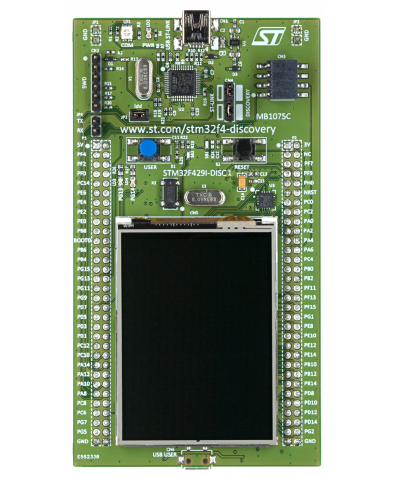
\includegraphics[width=0.6\textwidth]{discovery_kit}
    \caption{Комплект 32F429IDISCOVERY}
    \label{fig:discovery_kit}
\end{figure}

\subsubsection{Характеристики}

В следния списък са поместени основните характеристики
на микроконтролера \cite{stmmcudatasheet}.

\begin{itemize} 
    \item Ядро: \textit{32b Arm Cortex-M4} с FPU
    \item Максимална честота на процесора: 180MHz
    \item Флаш памет: 2048 Kbytes
    \item SRAM: Системна : 256 ( 112 + 16 + 64 + 64 ) Kbytes
    \item Таймери:
    \begin{itemize} 
        \item General Purpose: 10бр. (TIM2-5, TIM9-14)
        \item Advanced control: 2бр. (TIM1, TIM8)
        \item Basic: 2бр. (TIM6-7)
    \end{itemize}     
    \item Комуникационни интерфейси:
    \begin{itemize}
        \item SPI/I2S : 6/2 (пълен дуплекс) 
        \item I2C: 3
        \item USART/UART: 4/4
    \end{itemize} 
    \item GPIO: 114бр.
    \item Интерфейс за програмиране: \textit{ST-LINK}
    \item Опаковка: LQFP144 (\autoref{fig:mcu_pinout})
\end{itemize}



\begin{figure}[htpb!]
    \centering
    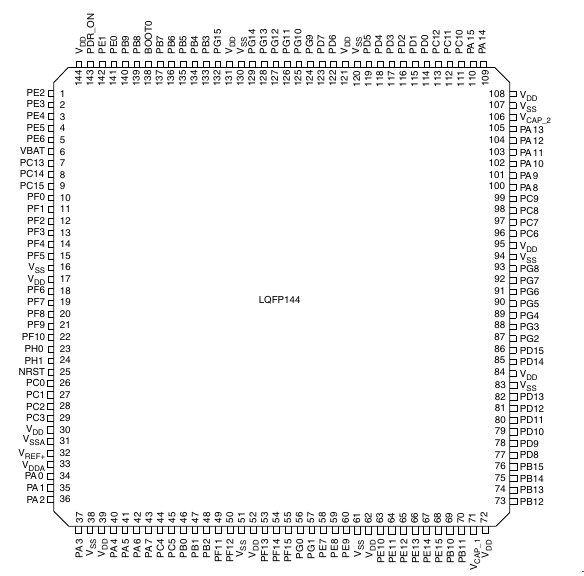
\includegraphics[width=0.6\textwidth]{mcu_pinout}
    \caption{Наименования на изведените пинове през използвания пакет}
    \label{fig:mcu_pinout}
\end{figure}

\subsubsection{Комплект 32F429IDISCOVERY}

Микроконтролерът е част от платка \textit{32F429IDISCOVERY} (\autoref{fig:discovery_kit})
(комплект за оценка на функционалиностите на \textit{STMicroelectronics}).
Комплектът предоставя множество функционалности, вградени в платката като
8MHz външен осцилатор, вграден \textit{ST-LINK} програматор,
LCD дисплей, 2 броя LED, както и удобна връзка към пиновете на
микроконтролера в THT формат.

Важно е да се отбележи, че в комплекта \textit{32F429IDISCOVERY}
има познат проблем с вградения \textit{ST-LINK} програматор.
Докато устройството не е свързано чрез USB, програматорът поддържа процесора в \textit{RESET}
през дебъгера.
Проблемът се решава, чрез ъпдейт на фърмуера на дебъгера 
или декуплиране чрез физическо разединяване на каналите на дебъгера върху платката (CN4). 

\FloatBarrier

